\cleardoublepage
\chapter{Hardware}\label{chap:hardware}
This chapter consists in the identification of the physical components to use in the solution to develop, from the proposed approach. It will be explained the selection of each one of them and their purpose in the system. Beside this will be briefly explain the hardware developed for signal conditioning and to stimulate the system. In the end, will be presented some methods to attach the sensors to the bottle.
\section{Selection}
This section presents the selection process of each sensor and its purpose in the application. What were the criteria to select the sensors to measure the vibration,  to process the data and to stimulate the system. 
\subsection{Microphone}
With the intent of understanding what is the system response to an external stimulation, is necessary a method to record that response. The easiest way to do that is by using a microphone to capture the sound produced, when hitting the side surface of the \acrshort{lpg} bottle.
The choice to use as a microphone was the one embedded in the phone. By the time the study started, was the most practical option available. The phone itself is connected via USB to the computer, on which additional software was installed to allow access in real time to the microphone of the phone.  
\subsection{Accelerometer}
As already mentioned in section \ref{sec:VibSens}, there are various types of accelerometers, however the choice depends on various factors. In this particular application is important that the accelerometer in use has a low cost and a small size, for the future application. With this in mind the choice declines over MEMS accelerometers, which are smaller when compared with piezoelectric accelerometers.

The type of \acrshort{mems} accelerometers available is very wide, some of them started to be used in applications that usually uses piezoelectric accelerometers, like condition-based monitoring, structural health monitoring, asset health monitoring, vital sign monitoring and \acrshort{iot}. When selecting the accelerometer it is important to take into consideration some parameters, which are responsible to determine the category of the accelerometer, their application, the bandwidth and the range. Although there is no standard for the category on each accelerometer fits in, \acrlong{ad} has one document where they divide their products in different categories, with the type of application where each one can be used, featuring a description of the key parameters, that must be taken into consideration when selecting the appropriate accelerometer~\cite{AnalogDialogue51102017}.
\begin{figure}[]
    \centering
    \includegraphics[width=1\textwidth]{Chapters/4CHP/Figures/adTable.pdf}
    \caption{Application landscape for a selection of Analog Devices MEMS accelerometers}
    \label{fig:adtable}
\end{figure}

The \acrshort{mems} accelerometers, from Analog Devices, are divided in two families, the ADXLxxxx and the ADIS16xxxx. The last offers different advantages when compared with the first, especially like a plug-and-play solution with features like factory compensation, embedded compensation and signal processing. This family has one of the features that has particular interest for the application, in this case the fact that it has signal processing on the accelerometer. On the other hand this family of products has a higher cost, which is not ideal if the final solution is suppose to be affordable. So it is necessary to define the key specifications of the accelerometer, in order to properly select one~\cite{AnalogDialogue51102017}.

The final purpose is to have a cheap and portable prototype, that is capable of accurately measuring the vibrations and determining the liquid level. This implies that the bandwidth covers the spectrum of frequency on which the curve of the relation liquid level vs frequency is. With this in mind the key specifications are the low cost, low power and his bandwidth. According to the results obtained by~\citeauthor{wuLiquidLevelDetector2014b}\cite{wuLiquidLevelDetector2014b} shown in section~\ref{sec:LPGModel} and the maximum frequency for a mechanical vibration, shown in table~\ref{tab:sampRat}, it can be used an accelerometer with a Bandwidth close to 2kHz. Considering these specification, some models where chosen, that integrate this criteria, as follows:
\begin{table}
    \centering
    \includegraphics[width=1\textwidth]{Chapters/4CHP/Figures/accTable.pdf}
    \caption{Key specifications of MEMS accelerometers}
    \label{tab:acctable}
\end{table}

Although it does not accommodate entirely the specifications, but since it was already available for use, the choice fell to the ADXL335. This model offers a low power consumption of around 350$\mu$A, its bandwidth is adjustable with a single capacitor per axis, from 0.5 to 1600 Hz for X and Y axis and 0.5 to 550 Hz for Z axis. Beside this the accelerometer itself is very cheap, with a price starting at 3€. To properly acquire the data from this sensor and process it, it is necessary to integrate it with an amplifier circuit and a microcontroller, on which more details will be explained further ahead.
\subsection{Piezoelectric}

There are several types of piezoelectric constituents, a defining factor of the type of material used in the piezoelectric, is his application. The most commonly used in vibration measurement is \acrshort{pvdf} as polymer and \acrshort{pzt} as ceramic. This sensor produces charges according to the applied pressure and the voltage generated at the output is related with the amount of charges generated. In a electric point a view, this is a sensor with a high-impedance, therefore is necessary a amplifier circuit with a high input impedance and with a high \acrshort{snr} relation. For piezoelectric it is usual to use a charge amplifier, that already fills these requirements.

In the developed work, two different piezoelectric were used, with different dimensions, one with a diameter of 27mm and the other with a diameter of 12mm.

\begin{figure}[]
    \centering
    \begin{subfigure}{0.45\textwidth}
        \centering
        \includegraphics[width=\linewidth]{Chapters/4CHP/Figures/piezo27mm.png}
        \caption{}{}
        \label{subfig:piezo1}
    \end{subfigure}
    \begin{subfigure}{0.45\textwidth}
        \centering
        \includegraphics[width=\linewidth]{Chapters/4CHP/Figures/piezo12mm.png}
        \caption{}{}
        \label{subfig:piezo2}
    \end{subfigure}
    \caption{Piezoelectric sensors used}{}
    \label{fig:UsedPiezos}
\end{figure}
The use of a piezoelectric is not only a cheaper option, when compared with the accelerometer, but also, allows to pursue a different approach. This is related to the stimulation technique of the system, that can replace the hitting to a different technique that uses the piezoelectric. 

\subsection{Microcontroller}
When selecting the microcontroller, it is important to have some specifications in mind, as in the perspective of a future implementation. Some are quite quite important, as the performance, the cost, as well as the power consumption. There is a large variety of products that most certainly would fit in these specifications. The selection of this it took in consideration those characteristics and fell to one from \acrlong{ti}. The model of the chosen, is the MSP-EXP430FR2433 and his characteristics are the following:
\begin{itemize}
    \item 16-bit \acrshort{risc} processor with a clock frequency up to 16MHz;
    \item 15KB of program and 512B information \acrshort{fram}, 4KB \acrshort{ram};
    \item 8-channel 10-bit \acrshort{adc};
    \item Four 16-bit Timers, 16-bit counter-only \acrshort{rtc};
    \item 32-bit Hardware-Multiplier;
    \item Two \acrshort{eusci}\_A, supports \acrshort{uart}, \acrshort{irda} and \acrshort{spi} and one \acrshort{eusci}\_B, supports \acrshort{spi} and \acrshort{i2c};
\end{itemize}
Beside these characteristics, the microcontroller offers different low-power modes, that consume from several hundreds of microAmps to a couple of hundreds of microAmps, depending on the mode of operation of the microcontroller. Another thing in consideration, when selecting, is the fact that it is possible to run with a super cap. The performance in this case is not as important as it seems as it is not mandatory that an operation that would need to be performed must return the result to the user instantly, that means that the results not being in real time will not make much of a difference anyway if that was the case. There is also a 32-bit Hardware-Multiplier embedded, that reduces the use of \acrshort{cpu} time to perform multiplications that would be required\cite{MSP430FR2433DataSheet}. Associated with these characteristics, the price of this microcontroller is very appealing, starting under 2€.

\subsection{Solenoid}
Since the use of the hammer to hit the bottle is not practical and has inconstant results, a solenoid will be used with the intention of substitute the hammer. This way, is possible to stimulate the system automatically by powering the solenoid. With that purpose the SOL01002 was selected because this solenoid works with voltages starting at 5V and the other reason is due the fact that is a Push type, which means that when powered the shaft will move and produce the desired impulse.
\begin{figure}[]
    \centering
    \includegraphics[width=0.45\textwidth]{Chapters/4CHP/Figures/solenoide.jpg}
    \caption{Solenoid used to stimulate the bottle}
    \label{fig:solenoid}
\end{figure}
The downside of using this model, can be the low impact force, it may not be able to produce a strong enough hit detectable by the sensors.
\section{Design}
This section is dedicated to explain how each circuit was planned to interact with the sensors in use, being important to the design what is the output of each signal. Before getting into details of each circuit, the resulting signal of each sensor and the consideration to further design the circuit will be presented.

\subsection{Accelerometer}
Considering that the accelerometer has three outputs, that are limited in frequency with a capacitor, the output used was the X axis with a bandwidth of 1600Hz, which is the maximum frequency.
\begin{figure}[]
    \centering
    \includegraphics[width=0.45\textwidth]{Chapters/4CHP/Figures/accTopView.pdf}
    \caption{Top view of ADXL335}
    \label{fig:topViewADXL}
\end{figure}

Considering the dot shown in the top view of the ADXL335, in figure~\ref{fig:topViewADXL}, when mounting the accelerometer in the side surface of the \acrshort{lpg} bottle, the dot is in the same position relative to the surface, on the top left corner. This way the output of the X axis measured, is around 1.25V, if the accelerometer is powered with 3.3V. Before designing the circuit to amplify the signal from the accelerometer is important to know, what should be the gain of the circuit. For that the surface of the bottle was hit with the hammer and the resulting output can be observed in figure~\ref{subfig:maxAccNDC}, approximately at the center of the image. In figure~\ref{subfig:maxAccN} is the same signal with zoom.

\begin{figure}[]
    \centering
    \begin{subfigure}{0.45\textwidth}
        \centering
        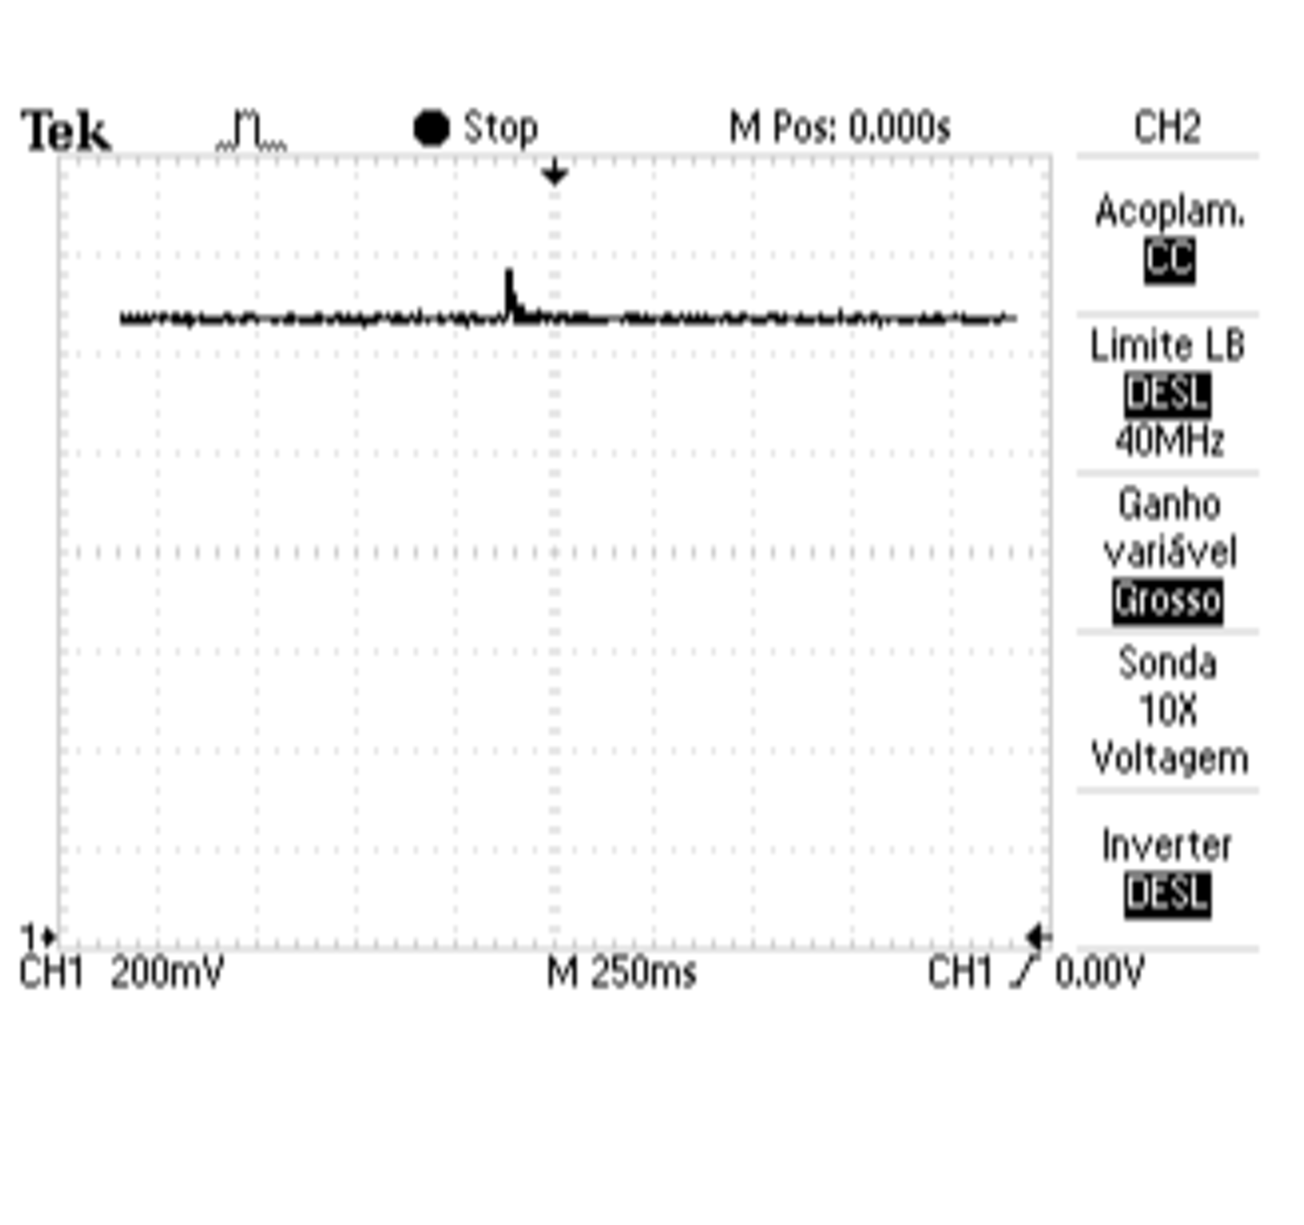
\includegraphics[width=\linewidth]{Chapters/4CHP/Figures/maxAccNDC.eps}
        \caption{Signal obtained after hitting in DC level}{}
        \label{subfig:maxAccNDC}
    \end{subfigure}
    \begin{subfigure}{0.45\textwidth}
        \centering
        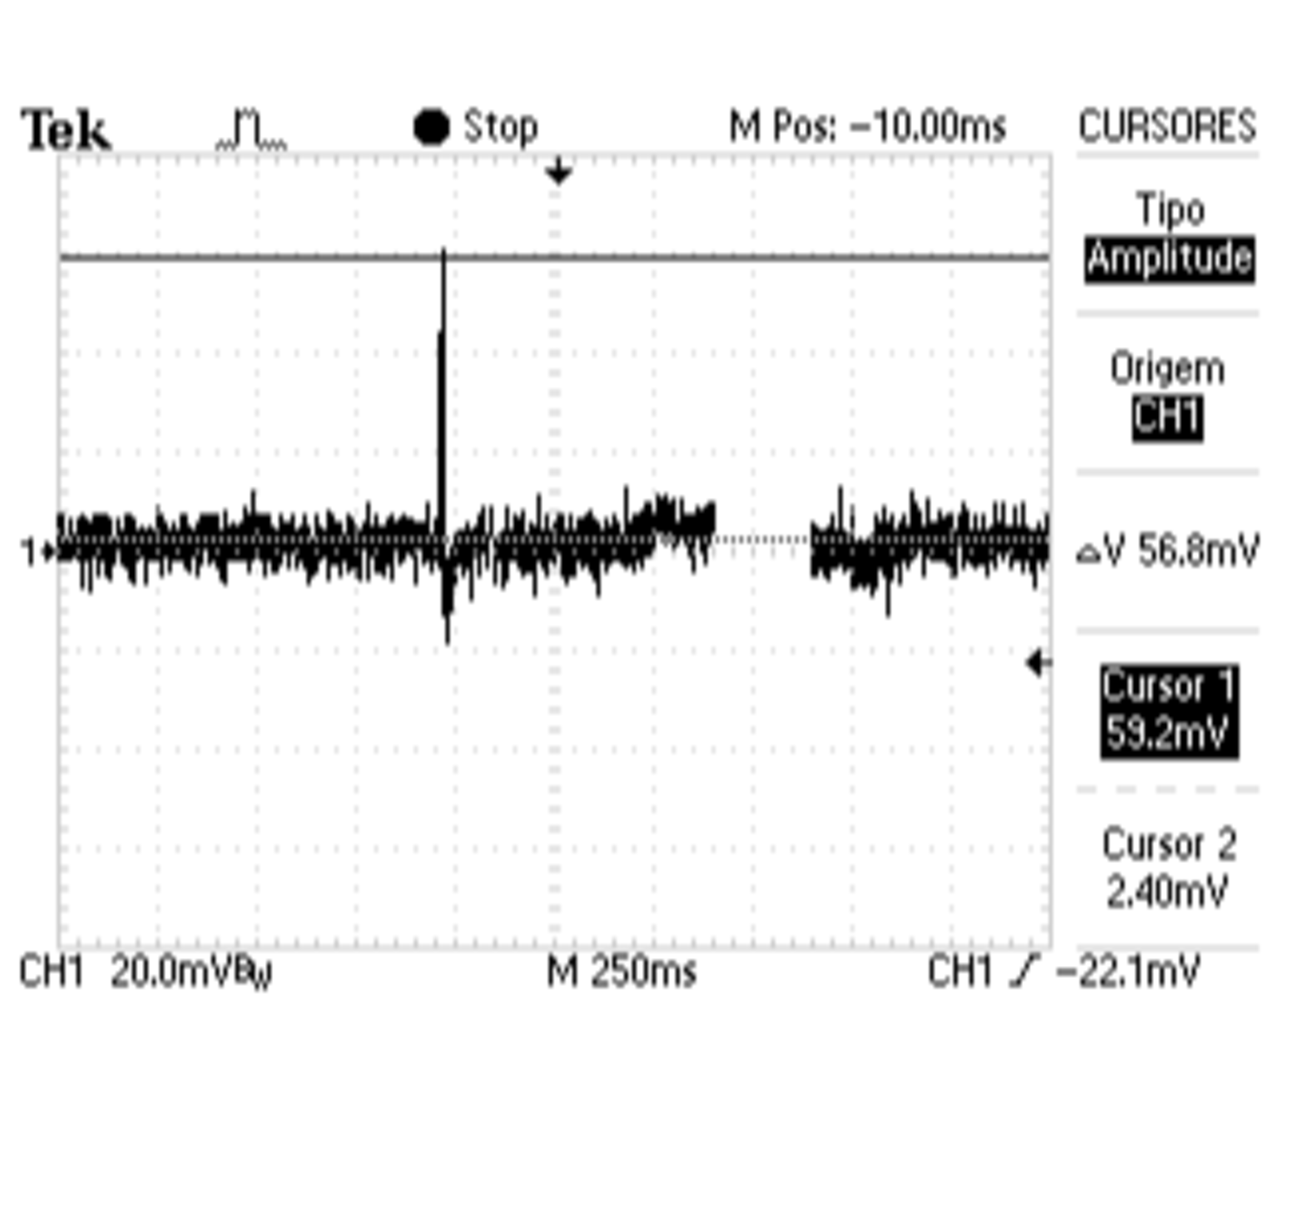
\includegraphics[width=\linewidth]{Chapters/4CHP/Figures/maxAccN.eps}
        \caption{Signal obtained after hitting, in AC}{}
        \label{subfig:maxAccN}
    \end{subfigure}
    \caption{Signal obtained in the accelerometer after hitting with the hammer}
    \label{fig:NampSigAcc}
\end{figure}

Considering that the output of the amplified signal should be between the supply voltage range, that is from 0-3.3V, being the minimum of the signal corresponding to one of the limits of the interval and the maximum to the other. If the amplifier circuit has an inverting configuration, the relation between the input and the output should be as illustrated in figure \ref{fig:inVSout}.
\begin{figure}[]
    \centering
    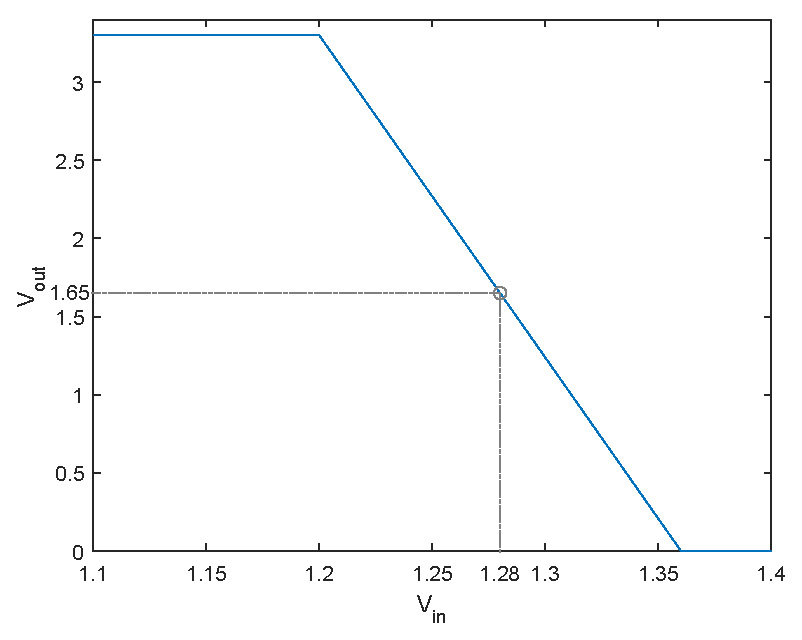
\includegraphics[width=0.45\textwidth]{Chapters/4CHP/Figures/inOut.eps}
    \caption{Desire relation between input and output of the amplifier circuit}
    \label{fig:inVSout}
\end{figure}

The gain of the circuit is determined in the following method:
\begin{equation}
   m = |\frac{\delta V_{Out}}{\delta V_{In}}| \approx |\frac{0-3.3}{1.3-1.2}| \approx 33
\end{equation}

In the equation, $m$ corresponds to the gain of the circuit, in this case only concerns is, the manual stimulation of the system. When changing to a automatic stimulation, is probable that the gain needs to be adjusted, considering the same procedure.

%%
A problem when design a proper circuit for this application is related with his supply voltage. Usually a amplifier circuit with an \acrshort{opamp}, the supply voltage is split, which means that the input/output signals are referenced to the ground. Since it will be used a battery or a super cap to power the device, limits us to a single supply.

In these situations, depending on the circuit configuration, the circuit may not operate for a determinate input voltage, since both input and output are referenced to the ground, thus the circuit will not function properly. In a dual supply voltage, if the supply voltages are symmetrical, the circuit is referenced to his midpoint, which is the ground. In a single supply it can be done in the same way, the signal can be referenced to half of the supply voltage, this is the simplest way to solve the presented problem. 

For now, to prove the concept, the circuit in use can be solved in the simplest way. In some situations and in a future application it may be needed to develop a robust solution for this. For those situations \acrshort{ti} provides a document that explains all the considerations that need to be taken into account and how to properly design the circuit for our application~\cite{manciniSingleSupplyOpAmp}.

As mentioned, to quickly test, is considered an inverting configuration is used to the amplifier circuit and the signal is referenced to the midpoint of the single supply voltage of the \acrshort{opamp}. As for the input signal, a capacitor is used in series to decouple from the DC level, this way the signal is "moved" to the midpoint between the supply voltage as referenced in the design from \acrshort{ti} in their document, providing a schematic for both non-inverting and inverting configuration~\cite{ACCoupledSingle2015}.

Figure~\ref{fig:accCircCom} shows the circuit used to amplify the signal from the accelerometer. Although the output of the accelerometer is around 1.25V, using the decoupling capacitor we are able to move the signal to the midpoint of the supply voltage. The only thing necessary is to adjust the gain of the circuit according to the desire relation between the input and output signals.
\begin{figure}[]
    \centering
    \begin{subfigure}{0.3\textwidth}
        \centering
        \includegraphics[width=\linewidth]{Chapters/4CHP/Figures/AmpAccCirc.pdf}
        \caption{}{}
        \label{subfig:AccAmpCirc}
    \end{subfigure}
    \begin{subfigure}{0.3\textwidth}
        \centering
        \includegraphics[width=\linewidth]{Chapters/4CHP/Figures/HalfSupply.pdf}
        \caption{}{}
        \label{subfig:VoltageDiv}
    \end{subfigure}
    \caption{Amplifiers circuit for accelerometer\ref{subfig:AccAmpCirc} and Midpoint supply voltage~\ref{subfig:VoltageDiv}}{}
\label{fig:accCircCom}
\end{figure}

\subsection{Piezoelectric}
As mentioned, piezoelectric sensors can be used in many fields, for sensing acceleration, vibration, shock or pressure. To what is related to acceleration or vibration, the piezoelectric will output a charge that is a function of his deformation/deflection. For the application in specific, the vibration produce, although is noticeable directly at the piezoelectric output, has a small amplitude which means that needs to be amplified to allow a distinct difference between what is actually the vibration and the output of the piezoelectric itself. To solve this, is important to properly design a signal conditioning amplifier circuit. \acrlong{ti} has a very clear document explaining how to design charge amplifiers for piezoelectric sensors~\cite{bartolomeSignalConditioningPiezoelectric2010}, on which they explain different types of circuits for this application in specific, with the advantages and disadvantages. The simplest model of this type of circuit is as follows~\ref{fig:ChargeAmpSimp}: 
\begin{figure}[]
    \centering
    \includegraphics[width=0.45\textwidth]{Chapters/4CHP/Figures/singleenddedchargeamp.pdf}
    \caption{Charge Amplifier for signal conditioning}
    \label{fig:ChargeAmpSimp}
\end{figure}

Two important things to consider is the bandwidth and the gain of the circuit. In the first case, the circuit functions as a High-Pass Filter which means that when selecting the feedback resistor and capacitance, their values must be selected to keep the cut off frequency low. The equation~\ref{eq:fhpf} can be used to define the cut off frequency.
\begin{equation}\label{eq:fhpf}
    f_{HPF} = \frac{1}{2\pi R_{FB}C_{FB}}
\end{equation}

Usually, the value of the resistor in use is on the order of hundreds of megaohms and the capacitance should be low. The reason is due to the fact that in these circuits the gain is defined by the value of the capacitance, the lower the value, the higher the gain~\ref{eq:gaincharge}.
\begin{equation}\label{eq:gaincharge}
    Gain = \frac{1}{C_{FB}} (mV/C)
\end{equation}

Another factor that must be taken in consideration is the \acrshort{snr}, which needs to be maximized. For this circuit in specific, one way to achieve this is by increasing the value of $R_{FB}$ as much as possible. To outline this and improve the \acrshort{snr} value, a differential charge amplifier is used.

\begin{figure}[]
    \centering
    \includegraphics[width=0.45\textwidth]{Chapters/4CHP/Figures/differentialchargeamp.pdf}
    \caption{Differential Charge Amplifier for signal conditioning}{\cite{bartolomeSignalConditioningPiezoelectric2010}}
    \label{fig:ChargeAmpDif}
\end{figure}

Since this types of circuit are very sensitive to interference, the differential charge amplifier offers one advantage when compared with the single-ended circuit. In the single-ended circuit in one of the inputs is injected current while the other is connected to the ground, this will amplify the interference. In the differential input the common-mode signals will cancel each other.

For the practical application, the  circuit in use will be as shown in figure \ref{fig:ChargeAmpDif}. Considering the simulation that the document \cite{bartolomeSignalConditioningPiezoelectric2010} presents, mainly those related with the \acrshort{snr}, this seemed to be the suitable choice for the application, since noise is a key aspect when measuring the signal, this is one way of reducing it. The difference in the circuit in use will be the components. The \acrshort{opamp} in use will be the MCP602 from Microchip, as for the remaining components, considering the information from the document, it can be select the values of 1nF for the capacitors and 100M$\Omega$ for the resistors. With these values, the cut off frequency of the High-Pass Filter will be set at 1,59Hz and the gain of the circuit 2G(V/C).
\begin{figure}[]
    \centering
    \includegraphics[width=0.45\textwidth]{Chapters/4CHP/Figures/piezoAmpcirc.PNG}
    \caption{Differential Charge Amplifier Schematic}
    \label{fig:ChargeAmpDifSCH}
\end{figure}

Note that, once again, beside being connected in differential mode, the circuit has on its positive input, a fixed input voltage of half the supply voltage of the \acrshort{opamp}.
\subsection{Solenoid}
The circuit needed for driving a solenoid is very simple, it consists simply of a \acrshort{mosfet}, a diode and a resistor as components. Is necessary to properly select the \acrshort{mosfet}, since if the solenoid is active by a microcontroller with a high output voltage of 3.3V in the specified pin, is necessary to have a low threshold voltage from the gate to the source. The use of the diode in parallel with the solenoid is to forward the current when the \acrshort{mosfet} is switched off. In figure~\ref{fig:solenoidshc} is the schematic of the circuit used to drive the solenoid.
\begin{figure}[]
    \centering
    \includegraphics[width=0.65\textwidth]{Chapters/4CHP/Figures/SolenoidDriver.PNG}
    \caption{Circuit for driving the solenoid}
    \label{fig:solenoidshc}
\end{figure}
\section{Capture/Coupling}\label{sec:CaptureCoupling}
This section is dedicated to present several techniques for mechanically attaching the sensors to the bottle. The coupling of the sensor to the bottle plays an important role in how the signal is sensed. In the end different techniques where selected to attach the sensor in use, to use in the tests chapter.
\subsection{Microphone}
To position the microphone and acquire the sound produced when hitting the tank surface, the microphone was placed perpendicular to the surface of the tank and as close as possible to it. The figure \ref{fig:micmount} is an illustration of how the microphone is placed relative to the \acrshort{lpg} bottle.
\begin{figure}[]
    \centering
    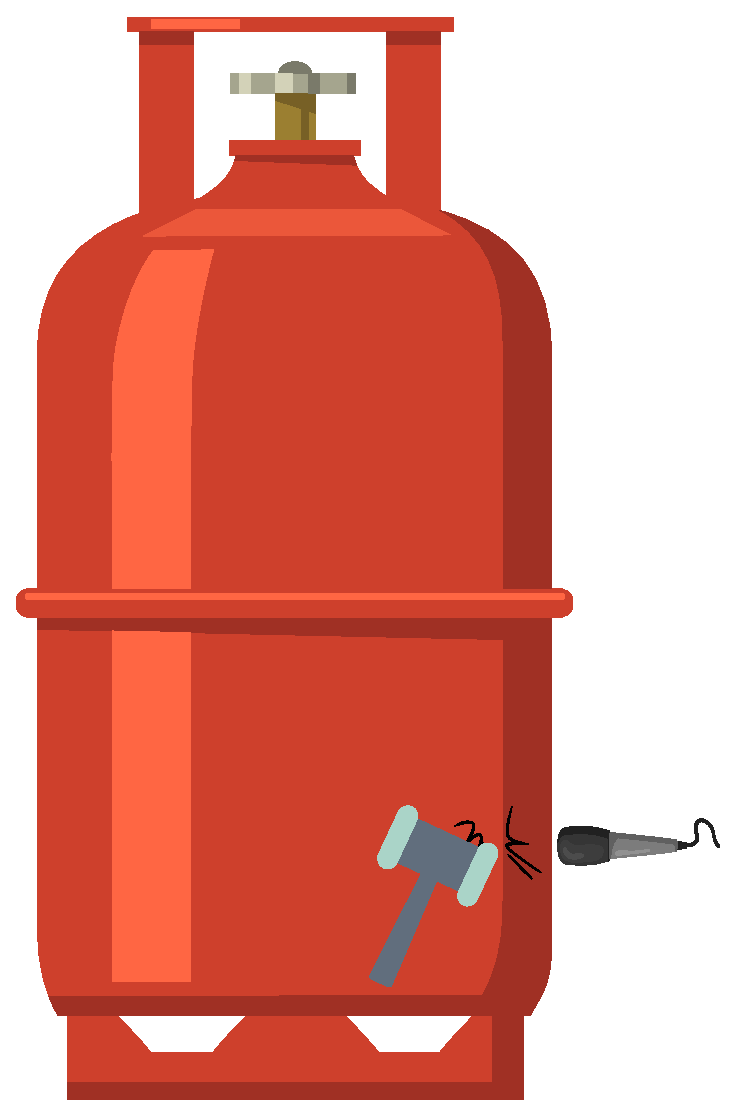
\includegraphics[width=0.3\textwidth]{Chapters/4CHP/Figures/micWimpactHamm.eps}
    \caption{Illustration of the accelerometer mount with a load strap}
    \label{fig:micmount}
\end{figure}
In the practical setup, since it uses the microphone from the phone, the side of the phone where the microphone is, should be faced to the \acrshort{lpg} bottle, usually the bottom part.
\subsection{Accelerometer}
When using an accelerometer for sensing vibration, there are different methods to mount it to the desired surface. In the industry, where accelerometers are used to measure vibrations of motors/machines, the accelerometer is mounted to the surface with a screw, allowing good contact with the surface. But in the application pretended is not possible to use that method, since that would imply the change in the structure of the tank and the accelerometer in use is not ready for a screw mount. Although the best results are obtained with a screw mount there are other methods to mount the accelerometer. 

One of the options is by using an adhesive, but in a practical mount the surface and the sensor would require different mounting bases, to avoid damaging the sensor and allow the sensor to be removed any time. Although this is practical to mount, it would also require that each tank already had the adhesive for the mount. The second option is a magnetic mount, offer a convenient mount if the structure of the tank is metallic. For this case it is advised that the magnet is in a separate piece, to avoid damaging the accelerometer. Magnets with a high pull strength are better in providing a good frequency response and a system with dual-magnet mount is good when the surface that the sensor is mounted on, is curve\cite{GuidelinesMountingTest}.

For the mount of the accelerometer in the \acrshort{lpg} bottle, will be used a magnet mount, is the most practical mount for a future application. Although in a laboratory environment and for test effects it will not be the only type of mount used. The first mount method will be with a load strap, this will hold firmly the sensor against the wall of the tank, as will be used for the first tests. In figure \ref{fig:mounLoadStrap} is an illustration of the sensor mount.

\begin{figure}[]
    \centering
    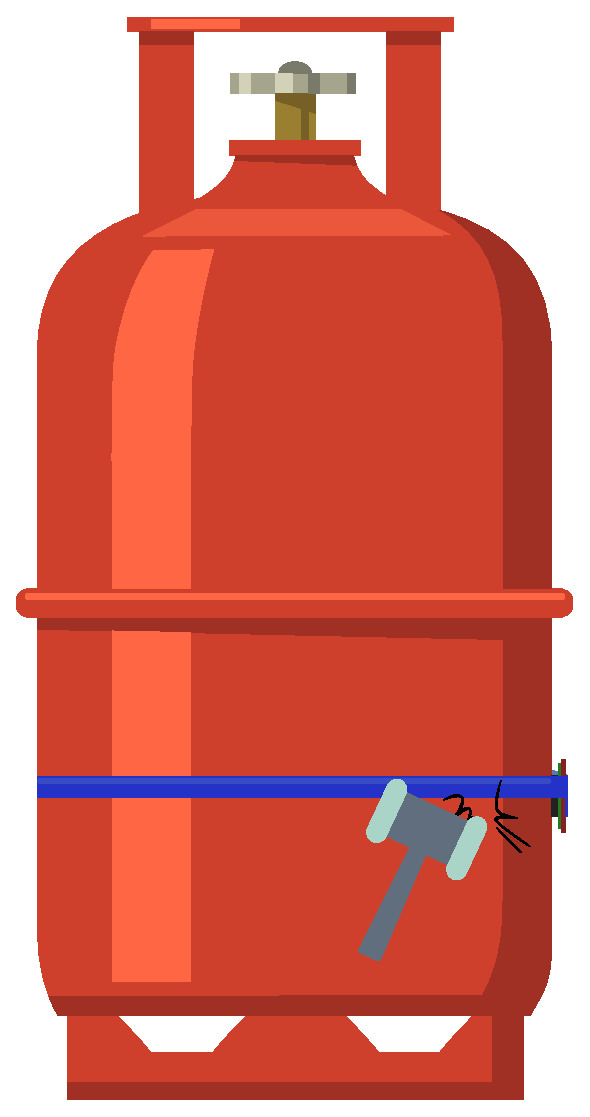
\includegraphics[width=0.3\textwidth]{Chapters/4CHP/Figures/AccLoadStrap.eps}
    \caption{Illustration of the accelerometer mount with a load strap}
    \label{fig:mounLoadStrap}
\end{figure}

For the magnet mount, there are actually two proposals, if by any reason one does not produce any results. In figure~\ref{subfig:mounMagnetDual} is the ideal option, since it is less invasive for the accelerometer, for the reason mentioned above. In this case, a piece is design to be able to mount with two neodymium magnets at the top and bottom of the piece, this will push the piece against the wall of the tank. Between the two magnets is the necessary space for held the accelerometer, a sponge will be glued to the piece on one side and the other will be glued to the accelerometer. This will be slightly thicker than the piece in that way when the magnets attached the piece against the tank wall, the sponge will be compressed and the surface of the accelerometer, is expected to be firmly held against the tank wall as well. In figure~\ref{subfig:mounMagnetsingle}, the mount is not ideal, since the neodymium magnet will be glued to the accelerometer surface for a god contact. This may result in better results when compared with the first option, but can damage the accelerometer, when attaching or removing the accelerometer from the tank wall.
\begin{figure}[]
    \centering
    \begin{subfigure}{0.3\textwidth}
        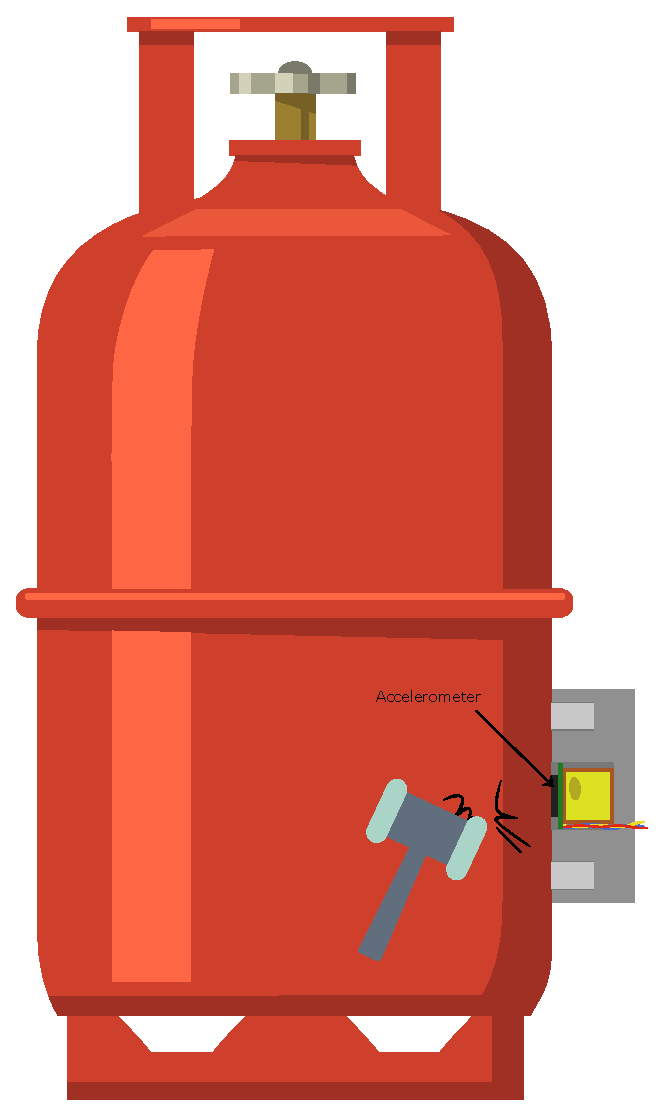
\includegraphics[width=\linewidth]{Chapters/4CHP/Figures/AccMagnets.eps}
        \caption{Illustration of dual-rail magnets mount}{}
        \label{subfig:mounMagnetDual}
    \end{subfigure}
    \begin{subfigure}{0.3\textwidth}
        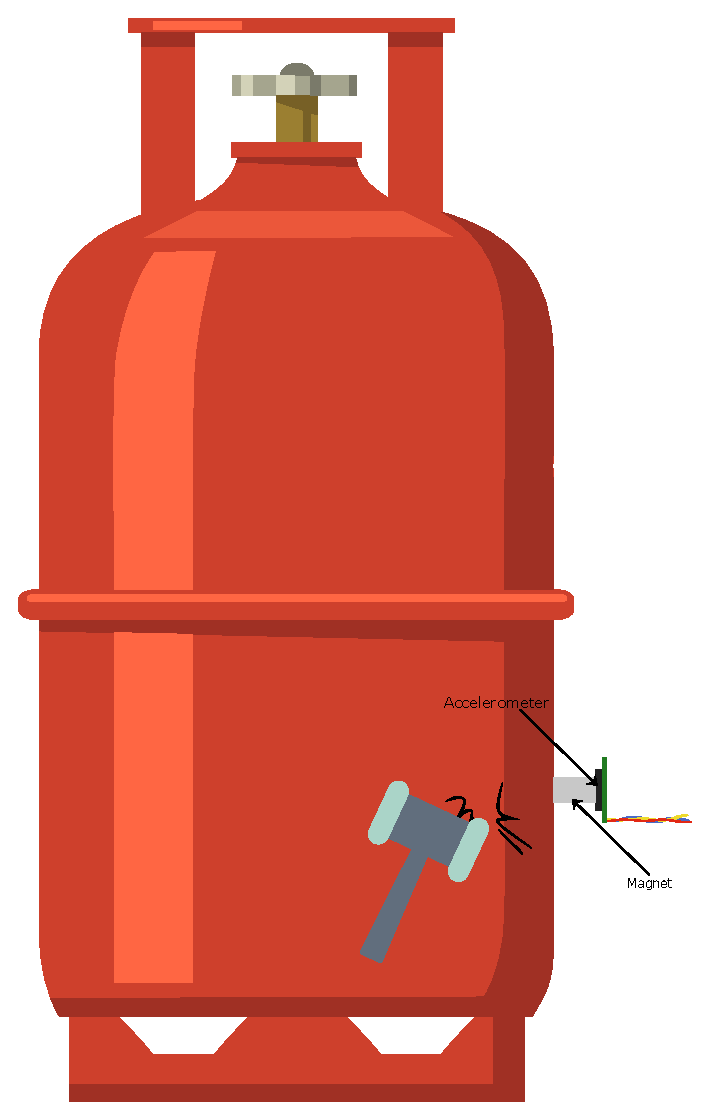
\includegraphics[width=\linewidth]{Chapters/4CHP/Figures/AccSMagnet.eps}
        \caption{Illustration of single magnet mount}{}
        \label{subfig:mounMagnetsingle}
    \end{subfigure}
    \caption{Illustration of the accelerometer mount with magnets}{}
    \label{fig:mounMagnet}
\end{figure}
%

\subsection{Piezoelectric}
\acrshort{ti} provides a document~\cite{minasiHowSelectMount2015}, with considerations for mounting a piezoelectric sensor to measure liquid level using ultrasonic waves. Although is a different approach, the key aspect for mounting this type of sensors can be used as well to define how to properly mount them. What needs to be taken into account, according to the document is, if the sensors is to be mounted inside or outside, at the top or at the bottom and for last the temperature range that the sensor can handles before starts to degrading the piezoelectric capability. It is quite clear the first aspect, since is suppose to be a non-invasive solution, which means that should be placed outside of the tank. The second aspect is not relevant since is being measured the vibration, not being used ultrasound to measure the liquid limit where the wave is reflected. The third aspect is also not that important since is expected to have the sensor at environment temperature unless, and this can be seen as an exception, when the gas from the tank has been release for a long period causing the outer wall of the bottle to freeze. Beside the first, which was already a requirement, none of the others will have a significant difference. For the purpose of measure through the walls of the tank is required to have a good contact between the transducer and the mounting surface. In their application the glue the transducer directly to the surface of the tank \cite{minasiHowSelectMount2015}.

Since the application is not ideal to have the transducer glued to the surface, the approach to have a good contact will be different, although the good results are not guaranteed. The figure \ref{fig:coupPiezo} is the illustration of two different mounting pieces for the transducer.
\begin{figure}[]
    \centering
    \begin{subfigure}{0.3\textwidth}
        \centering
        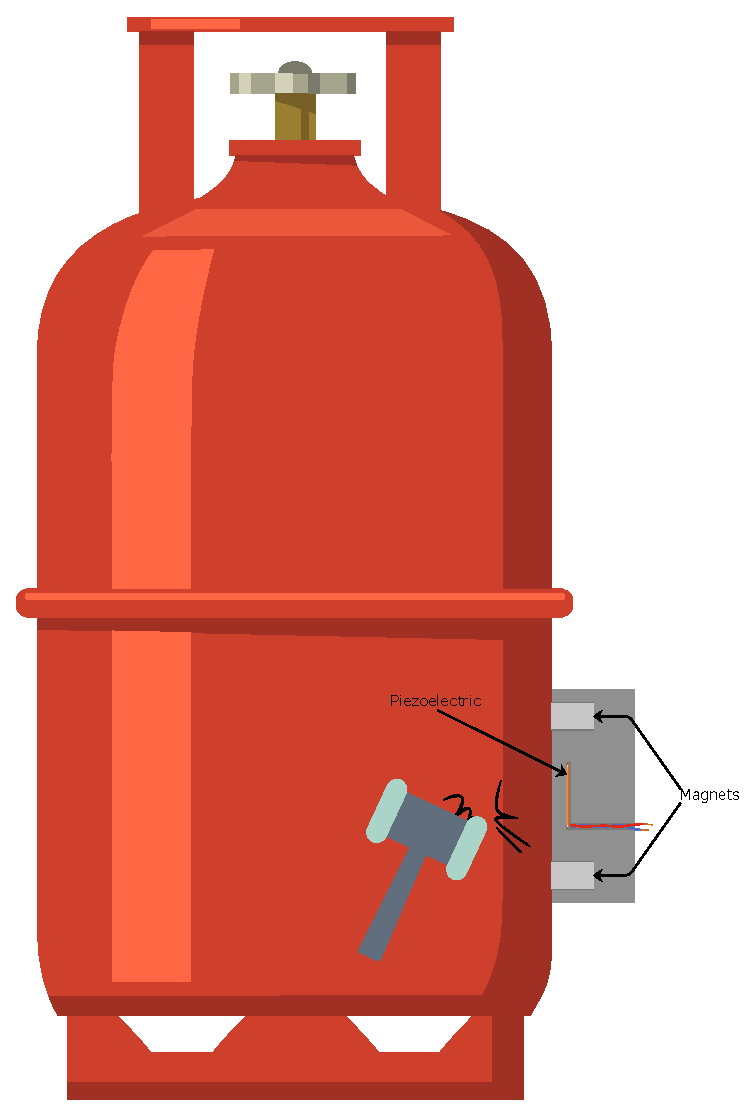
\includegraphics[width=\linewidth]{Chapters/4CHP/Figures/PiezoMagnetsSlot.eps}
        \caption{}{}
        \label{subfig:piezoslot}
    \end{subfigure}
    \begin{subfigure}{0.3\textwidth}
        \centering
        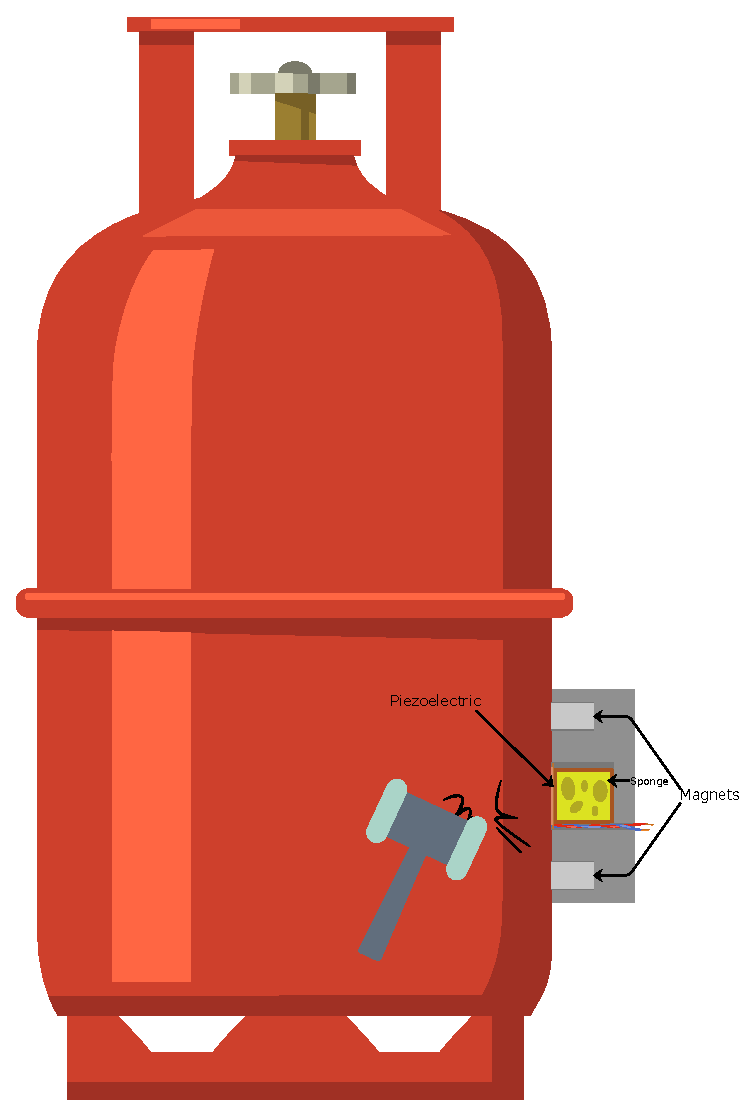
\includegraphics[width=\linewidth]{Chapters/4CHP/Figures/PiezoMagnets.eps}
        \caption{}{}
        \label{subfig:piezosponge}
    \end{subfigure}
    \caption{Illustration of the piezoelectric mount with magnets}{}
    \label{fig:coupPiezo}
\end{figure}

Both pieces will stay held to the tank with two magnets, one at the top of the piece and the other at the bottom. In figure \ref{fig:coupPiezo}~\subref{subfig:piezoslot}, the transducer is embedded in the piece, there is a slot in the middle, when the entire piece vibrates, the transducer vibrates with it. In the figure \ref{fig:coupPiezo}~\subref{subfig:piezosponge}, the coupling of the transducer is different when compared with the first one presented, the transducer is held glued to a sponge, and the sponge to the piece. The sponge is larger than the hole where the piece is glued in, so when the entire piece is attached to the walls of the tank, with the help of the magnets, it guarantees a good contact of the transducer with the wall. Since the sponge will press it against the wall and when there is vibration in the wall of the tank, it is expected to the transducer to capture the actual vibration. 

\section{Concluding remarks}
The current chapter presented the hardware parts and the physical components of the architecture presented to the system. The selection/design of the elements was based in already known concepts of electronics, properly justified, in most of the cases, with existing documentation about the topic.

The presented elements of hardware were either produced or prepared, to use in the step that follow this, i.e. the selected sensors were attached using the mentioned coupling methods, and the schematics presented were printed in a \acrshort{pcb}(\acrlong{pcb}), to use to drive required components of the system. These elements will later be part of the tests set, along with the software elements that will be explored in the next chapter.

\clearpage